\documentclass[letterpaper,10pt]{article}
\usepackage[top=2cm, bottom=1.5cm, left=1cm, right=1cm]{geometry}
\usepackage{amsmath, amssymb, amsthm,graphicx}
\usepackage{fancyhdr}
\pagestyle{fancy}

\lhead{\today}
\chead{Regression Assignment 6a}
\rhead{Justin Hood}

\newcommand{\Z}{\mathbb{Z}}
\newcommand{\Q}{\mathbb{Q}}
\newcommand{\R}{\mathbb{R}}
\newcommand{\C}{\mathbb{C}}
\newtheorem{lem}{Lemma}

\begin{document}
We shall fit a regression of the form,
\[y_t=\beta_0+\beta_1 t+\beta_2 Q_2+\beta_3 Q_3+\beta_4 Q_4+\epsilon_t\]
With $Q_i$ dummy variables for the $i^{th}$ quarter of a given year. 
\begin{enumerate}
\item First, we define the dummy variables as follows.
\begin{align*}
Q_2 &= \begin{cases}
1 & t\in\text{Quarter 2}\\
0 & t\not\in\text{Quarter 2}
\end{cases}\\
Q_3 &= \begin{cases}
1 & t\in\text{Quarter 3}\\
0 & t\not\in\text{Quarter 3}
\end{cases}\\
Q_4 &= \begin{cases}
1 & t\in\text{Quarter 4}\\
0 & t\not\in\text{Quarter 4}
\end{cases}
\end{align*}
\item Next, we plot the data to analyze the overall data trends to see if we need to scale for constant seasonal variation.
\begin{center}
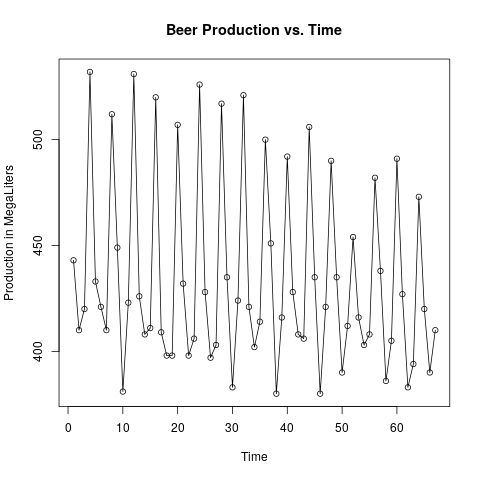
\includegraphics[scale=.8]{unlogged.png}
\end{center}
We see here that the overall trend of the data is negative, but there is no major increase or decrease in seasonal variation over the experimental region. As such, we expext $\beta_1$ to have a negative value, and we will not log or scale the $y$ variable at all to approximate constant variation.
\item We now construct our prediction equation and approximate,
\begin{tabular}{|c|c|}
\hline
$y_*$ & Prediction \\\hline
$y_{68}$ & $491.31$ \\


\end{tabular} 
\end{enumerate}
\end{document}
